%-----------------------------------------------------------------------------
%
%          PHYSICS  M.S.     THESIS
%          JUSTIN A. VASEL
%
%          This began as the template offered by the University of Minnesota, 
%          but I've made a few changes here and there...  
%
%          -->  thesis.tex
%
%-----------------------------------------------------------------------------



%-------------------------------------------------------------------------------
%    //  P R E A M B L E
%===============================================================================
	\documentclass[12pt, twoside, fleqn]{mnthesis}
	
	%%%%%%%%%%%%%%%%%%%%%%%%%
	%   //  PACKAGES        %
	%%%%%%%%%%%%%%%%%%%%%%%%%
		% // EPS Files
			\usepackage{epsfig}
			\usepackage{epic}
			\usepackage{eepic}

		% // Graphics and Figures
			\usepackage{graphicx}
			\usepackage{float}
			\usepackage[font=small]{caption}
			\usepackage{subcaption}
			\usepackage{wrapfig}

		% // TikZ
			\usepackage[usenames,dvipsnames]{xcolor}
			\usepackage{tikz}
			\usetikzlibrary{decorations.pathmorphing,decorations.markings,trees}		% Needed for Feynman diagrams
			\pgfdeclarelayer{background}
			\pgfdeclarelayer{foreground}
			\pgfsetlayers{background,main,foreground}

		% // Tables
			\usepackage{array}
			\usepackage{multirow}
			\usepackage{longtable}
			\usepackage{booktabs}

		% // Maths
			\usepackage{amsmath}
			\usepackage{amssymb}
			\usepackage{mathrsfs}

		% // HEP
			\usepackage{braket}			% Dirac notation
			\usepackage{hepparticles}	% Format particle processes
			\usepackage{hepnames}		% Format particle names
			%\usepackage{hepunits}		% Format HEP units

		% // Hyperlinks
			\usepackage[colorlinks=true, urlcolor=BrickRed, linkcolor=Black, citecolor=Black]{hyperref}		% href
			\usepackage{url}			% Don't use, makes text unicode

		% // Misc.
			\usepackage[emulate=hepunits,sepfour=true,digitsep=comma]{siunitx}		% Handles unit formatting
				\DeclareSIUnit\year{yr}
			\usepackage{lipsum}			% Generate Lorem Ipsum text
			\usepackage{setspace}
			\usepackage{titlesec}
			\usepackage[leftmargin=2in,rightmargin=0in,vskip=0.5in]{quoting}
			%\usepackage{indent first}
			\usepackage{lettrine}
			\usepackage{lineno}

		% // Unknown
			\usepackage{bigstrut}		% No idea what this does


	%%%%%%%%%%%%%%%%%%%%%%
	%   //  FONTS        %
	%%%%%%%%%%%%%%%%%%%%%%

		% // fontenc may be redundant. fontspec needed to use system fonts
		\usepackage[T1]{fontenc}
		\usepackage{fontspec}
		\usepackage{anyfontsize}

		% // Required in XeLaTeX to make system fonts have TeX ligatures
		%\defaultfontfeatures{Ligatures=TeX}

		% // Set the default document font to `Baskerville'
		%\setmainfont{Baskerville}
		\setmainfont[Mapping=tex-text,Ligatures={Historical}]{Adobe Caslon}

		% // DEFINE \neue as `Helvetica Neue'
		% // DEFINE \light as `Helvetica Neue UltraLight'
		% // DEFINE \minion as `Minion Pro'
		%\newfontfamily\garamond[]{Goudy Old Style}
		\newfontfamily\garamond[]{Medio}
		\newfontfamily\neue[]{Helvetica Neue}
		\newfontfamily\light[]{Helvetica Neue UltraLight}
		\newfontfamily\minion[]{Minion Pro}
		\newfontfamily\caslon[]{Adobe Caslon Pro}
		\newfontfamily\bask[]{Baskerville}

		% // Custom formatting for chapter titles
		\titleformat{\chapter}[display]{\nolinenumbers \raggedright \linespread{0.5} \huge}{\chaptertitlename\ \vspace{0.25in} \thechapter}{0pt}{\fontsize{40}{50}\selectfont}
		
		% // Custom formatting for captions
		\DeclareCaptionLabelFormat{smallcaps}{\normalsize \minion \textsc{#1 #2}}
		\captionsetup[figure]{name=Fig.}
		\captionsetup{labelformat=smallcaps, labelfont=bf, labelsep=period}



	%%%%%%%%%%%%%%%%%%%%%%
	%   //  GRAPHICS     %
	%%%%%%%%%%%%%%%%%%%%%%
		
		% // Set path to look for images and graphics extension types
		\graphicspath{ {../images/}{../images/Intro/}{../images/Neutrinos/}{../images/Supernovae/}{../images/Snews/}{../images/Halo/}{../images/Conclusion/} }
		\DeclareGraphicsExtensions{.eps,.pdf,.png}
		
		
		
	%%%%%%%%%%%%%%%%%%%%%%
	%   //  OTHER        %
	%%%%%%%%%%%%%%%%%%%%%%

		% // Pull in custom definitions
		%-----------------------------------------------------------------------------
%
%          PHYSICS  M.S. THESIS
%          JUSTIN A. VASEL
%
%          -->  TeX/Definitions/my_definitions.tex
%
%          This began as the template offered by the University of Minnesota, 
%          but I've made a few changes here and there...  
%
%-----------------------------------------------------------------------------

%% MATHS
    \newcommand{\COS}{{\mathrm{cos}}}
    \newcommand{\SIN}{{\mathrm{sin}}}


%% UNITS
    % energy (prefix: e)
    \newcommand{\eGeV}[1]{\SI{#1}{\GeV}}
    \newcommand{\eMeV}[1]{\SI{#1}{\MeV}}
    \newcommand{\ekeV}[1]{\SI{#1}{\keV}}
    \newcommand{\eeV}[1]{\SI{#1}{\eV}}

    % mass (prefix: m)
    \newcommand{\mGeV}[1]{\SI[per=slash,eVcorrb=0.4ex]{#1}{\giga\eVperc\squared}}
    \newcommand{\mMeV}[1]{\SI[per=slash,eVcorrb=0.4ex]{#1}{\mega\eVperc\squared}}
    \newcommand{\mkeV}[1]{\SI[per=slash,eVcorrb=0.4ex]{#1}{\kilo\eVperc\squared}}
    \newcommand{\mmeV}[1]{\SI[per=slash,eVcorrb=0.4ex]{#1}{\eVperc\squared}}


%% HEADINGS
    \newcommand{\CONT}{\noindent}
    \newcommand{\FIG}{Fig. \nolinebreak }
    \newcommand{\FIGS}{Figs. \nolinebreak }
    \newcommand{\SEC}{Sec.\ }
    \newcommand{\SECS}{Secs.\ }
    \newcommand{\TAB}{Table }
    \newcommand{\TABS}{Tables }
    \newcommand{\EQ}{Eq.\nolinebreak \ }
    \newcommand{\EQS}{Eqs.\nolinebreak \ }
    \newcommand{\APP}{Appendix }
    \newcommand{\APPS}{Appendices }
    \newcommand{\CHP}{Chapter }
    \newcommand{\CHPS}{Chapters }


%% OTHER
    % Small caps use Minion font
    \newcommand{\scaps}[1] {
    	\minion \textsc{#1}\normalfont
    }

    % Customized Lettrine environment for text at beginning of chapter
    \newcommand{\chapterIntro}[2] {
    	\noindent
    	\lettrine[lines=4,nindent=4pt]{#1}{\scaps{#2}}
    }

    % Makes it easier to typeset He-3 
    \newcommand{\he}{$^3$He}

    % Customize syntax highlighting for JSON & Obj-C
    \colorlet{punct}{red!60!black}
    \definecolor{background}{HTML}{EEEEEE}
    \definecolor{delim}{RGB}{20,105,176}
    \colorlet{numb}{magenta!60!black}

    \lstdefinelanguage{json}{
        basicstyle=\footnotesize\ttfamily,
        stepnumber=1,
        numbersep=8pt,
        showstringspaces=false,
        extendedchars=\true,
        frame=lines,
        backgroundcolor=\color{background},
        literate=
         *{0}{{{\color{numb}0}}}{1}
          {1}{{{\color{numb}1}}}{1}
          {2}{{{\color{numb}2}}}{1}
          {3}{{{\color{numb}3}}}{1}
          {4}{{{\color{numb}4}}}{1}
          {5}{{{\color{numb}5}}}{1}
          {6}{{{\color{numb}6}}}{1}
          {7}{{{\color{numb}7}}}{1}
          {8}{{{\color{numb}8}}}{1}
          {9}{{{\color{numb}9}}}{1}
          {:}{{{\color{punct}{:}}}}{1}
          {,}{{{\color{punct}{,}}}}{1}
          {\{}{{{\color{delim}{\{}}}}{1}
          {\}}{{{\color{delim}{\}}}}}{1}
          {[}{{{\color{delim}{[}}}}{1}
          {]}{{{\color{delim}{]}}}}{1},
    }

    \lstdefinelanguage{object-c}{
        basicstyle=\footnotesize\ttfamily,
        stepnumber=1,
        numbersep=8pt,
        showstringspaces=false,
        extendedchars=\true,
        frame=lines,
        backgroundcolor=\color{background},
        literate=
         *{0}{{{\color{numb}0}}}{1}
          {1}{{{\color{numb}1}}}{1}
          {2}{{{\color{numb}2}}}{1}
          {3}{{{\color{numb}3}}}{1}
          {4}{{{\color{numb}4}}}{1}
          {5}{{{\color{numb}5}}}{1}
          {6}{{{\color{numb}6}}}{1}
          {7}{{{\color{numb}7}}}{1}
          {8}{{{\color{numb}8}}}{1}
          {9}{{{\color{numb}9}}}{1}
          {:}{{{\color{punct}{:}}}}{1}
          {,}{{{\color{punct}{,}}}}{1}
          {=}{{{\color{punct}{=}}}}{1}
          {"}{{{\color{punct}{"}}}}{1}
          {@}{{{\color{punct}{@}}}}{1}
          {\{}{{{\color{delim}{\{}}}}{1}
          {\}}{{{\color{delim}{\}}}}}{1}
          {[}{{{\color{delim}{[}}}}{1}
          {]}{{{\color{delim}{]}}}}{1}
          {)}{{{\color{delim}{)}}}}{1}
          {(}{{{\color{delim}{(}}}}{1},
    }


%-----------------------------------------------------------------------------
%-----------------------------------------------------------------------------

		% // Set linespacing for document
		\linespread{1.3}

		% // Algin all math environs to left side
		\setlength{\mathindent}{0cm}




%-------------------------------------------------------------------------------
%    //  B E G I N   D O C U M E N T
%===============================================================================
	\begin{document}
	
	% // Decoration for Feynman digram symbols
	\tikzset{
	    photon/.style={
		    decorate, 
		    decoration={snake}, 
		    draw=red
		},
	    fermion-in/.style={
	    		draw=black, 
			postaction={decorate},
	        decoration={
	        		markings,
				mark=at position .55 with {\arrow[draw=black]{<}}
			}
		},
		fermion-out/.style={
	    		draw=black, 
			postaction={decorate},
	        decoration={
	        		markings,
				mark=at position .55 with {\arrow[draw=black]{>}}
			}
		},
	    gluon/.style={
	    		decorate, 
			draw=magenta,
	        decoration={
	        		coil,
				amplitude=4pt, 
				segment length=5pt
			}
		} 
	}
	
	% // Show all cite & un-cited references
	%\nocite{*}


	%%%%%%%%%%%%%%%%%%%%%%%%%%%%%%%
	%   //  BUILD DOCUMENT        %
	%%%%%%%%%%%%%%%%%%%%%%%%%%%%%%%

		%\frontmatter		
		% // Frontmatter
			%-----------------------------------------------------------------------------
%
%          PHYSICS  M.S.     THESIS
%          JUSTIN A. VASEL
%
%          This began as the template offered by the University of Minnesota, 
%          but I've made a few changes here and there...  
%
%          -->  title.tex
%
%-----------------------------------------------------------------------------


% For a  PhD give the command \phd. Default is masters
%\degree (normally Doctor of Philosophy or Master of Science)
%\initials (normally Ph.D. or M.S.)
\ms % use if for a Master of Science thesis
%\phd % use if for a Ph.D. dissertation
%\draft

\title{\fontsize{45}{60}\selectfont\garamond UNDER THE HOOD \normalfont \normalsize  \\ \vspace{0.1in} \large \light \emph{Preparing the Helium and Lead Observatory for Full Operation} \normalfont \normalsize}
\author{Justin A. Vasel}
\campus{University of Minnesota Duluth} 
\program{Physics} 
\director{Dr. Alec Habig} 

% Optionally specify the month and year.
\submissionmonth{August} % defaults to current month.
\submissionyear{2013} % defaults to current year.

%Comment out below on final copy
\abstract{%%%%%%%%%%%%%%%%%%%%%%%%%%%%%%%%%%%%%%%%%%%%%%%%%%%%%%%%%%%%%%%%%%%%%%%%%%%%%%%%
% abstract.tex: Abstract
%%%%%%%%%%%%%%%%%%%%%%%%%%%%%%%%%%%%%%%%%%%%%%%%%%%%%%%%%%%%%%%%%%%%%%%%%%%%%%%%

The Helium and Lead Observatory (HALO) at SNOLAB in Canada is the world's first dedicated supernova neutrino detector. Construction of the detector is complete, but there is still work to be done before it is fully operational. In this thesis, I describe my contributions to the HALO experiment which include the testing of hardware, the design of a redundant networking scheme, and the development and implementation of a remote monitoring system.

%%%%%%%%%%%%%%%%%%%%%%%%%%%%%%%%%%%%%%%%%%%%%%%%%%%%%%%%%%%%%%%%%%%%%%%%%%%%%%%%
}
\words{331}    % number of words in the abstract
\copyrightpage % Do you want copyright protection?
\acknowledgements{%-----------------------------------------------------------------------------
%
%          PHYSICS  M.S.     THESIS
%          JUSTIN A. VASEL
%
%          This began as the template offered by the University of Minnesota, 
%          but I've made a few changes here and there...  
%
%          -->  acknowledge.tex
%
%-----------------------------------------------------------------------------



\chapterIntro{G}{raduate work is demanding.} It requires the student to utilize or develop many attributes; autonomy, dedication, discipline, and perseverance are a few. But, a successful post-graduate career also requires a strong support structure, on both a professional and personal level. 

There are many people that have earned my gratitude for their contribution to my success in graduate school. Dr. Alec Habig has been invaluable as a mentor. He taught me what it means to be an experimenter, and helped me stay afloat as I waded into the waters of particle physics for the first time.

Dr's. Clarence Virtue and Michael Shumacker of Laurentian University in Ontario also deserve my thanks. Their kindness and guidance made coming to an intimidating laboratory in a country I had never been to a peaceful and enjoyable experience. Being part of bringing the HALO experiment from partial-completion to near-completion has been a rewarding experience; I am grateful to have worked on a project that will someday help make historical observations.

But, perhaps there are none more deserving of my gratitude than my parents, Steve Vasel and Jennifer Olson.  


%-----------------------------------------------------------------------------
%-----------------------------------------------------------------------------}
\dedication{To my mother and father, who taught me of the world. 

}
\abbreviations{%-----------------------------------------------------------------------------
%
%          PHYSICS  M.S.     THESIS
%          JUSTIN A. VASEL
%
%          This began as the template offered by the University of Minnesota, 
%          but I've made a few changes here and there...  
%
%          -->  colophon.tex
%
%-----------------------------------------------------------------------------

\begin{minipage}{0.7\textwidth}
	\onehalfspacing
	\minion
	\large
	\raggedright\lettrine[lines=2,slope=-2pt,nindent=-4pt]{\textcolor{BrickRed}T}{his thesis was typeset} with \LaTeX, using the mnthesis document class. The body text is set in 12 point Baskerville, designed by John Baskerville in 1757. The caption labels are set in 12 point Minion with small caps. The original template is available publicly at the University of Minnesota, and the modified version used to produce this document can be found online at \href{http://github.com/justinvasel/}{http://github.com/justinvasel} or directly from the author at \href{mailto:justin.vasel@gmail.com}{justin.vasel@gmail.com}.
	\normalsize
	\normalfont
\end{minipage}

%-----------------------------------------------------------------------------
%-----------------------------------------------------------------------------}

% Use a special preface
%\extra{\input{preface}}

% The \beforepreface command actually causes insertion of the title, 
% abstract, signature, and copyright pages into the new document.
\beforepreface 

% Define the text to go before the table of contents
\figurespage
\tablespage

% The \afterpreface command actually causes insertion of the
% contents, list of figures, etc. into the new document.
\afterpreface            


%-----------------------------------------------------------------------------
%-----------------------------------------------------------------------------

		%\mainmatter
		% // Background
			%\linenumbers
			
			\cleardoublepage % // Ensures each chapter starts on a right-handed page
			%-----------------------------------------------------------------------------
%
%          PHYSICS  M.S.     THESIS
%          JUSTIN A. VASEL
%
%          This began as the template offered by the University of Minnesota, 
%          but I've made a few changes here and there...  
%
%          -->  intro.tex
%
%-----------------------------------------------------------------------------


\chapter{Introduction}
	\label{intro_chapter}
	\vspace{-0.2in}

	\begin{quoting}
		\noindent \large ``Measure what is measurable, and make measurable what is not so." \normalsize

		--- Galileo Galilei
	\end{quoting}

	Nothing...


	



%-----------------------------------------------------------------------------
%-----------------------------------------------------------------------------

			
			\cleardoublepage
			%-----------------------------------------------------------------------------
%
%          PHYSICS  M.S.     THESIS
%          JUSTIN A. VASEL
%
%          This began as the template offered by the University of Minnesota, 
%          but I've made a few changes here and there...  
%
%          -->  neutrinos.tex
%
%-----------------------------------------------------------------------------


\chapter{The Physics of Neutrinos}
	\label{neutrino_physics_chapter}

	\vspace{-0.2in}

	\begin{quoting}
		\noindent \large ``Neutrinos, they are very small." \normalsize

		--- John Updike
	\end{quoting}

	\chapterIntro{T}{he turn of the twentieth century} marked the beginning of a golden age in physics. The formulation of relativity and formalism of quantum mechanics brought with it a wealth of paradigm-shifting discoveries, offering humanity a deeper, more fundamental understanding of the Universe and paving the way for decades of ground-breaking research. One of the crowning achievements of this era has been the construction of the Standard Model of particle physics.

	The advent of the model was paramount to the advancement of modern physics. Through its theoretical framework, the particle physicist can calculate, among other things: decay modes, branching ratios and intrinsic properties of a myriad of particles. In some instances, the very existence of yet unobserved particles can be inferred from the Standard Model. The prediction of the Higgs boson---whose existence was proposed to preserve gauge invariance---is perhaps the most notable example, being initially theorized in 1964 and finally discovered in March 2013.

	It is essential in particle physics that one be able to predict the observed phenomena before it is observed. While atomic particles like the proton, neutron, and electron are easy to detect, many particles are not. This is especially true for particles that have a low mass or no charge, like the neutrino, or very brief lifetimes like the Higgs boson. It is nearly impossible to detect these particles directly. Instead, one must depend on indirect observations like the products of an interaction or the daughter particles of a decay sequence. To make new discoveries, the particle physicist must know what she is looking for and where she might find it; it is the nature of the beast. 

	\section{The Standard Model of Particles}

	The Standard Model of Particles is the result of large-scale scientific collaboration, spanning several continents and decades. Feynman said in his famous recorded lectures on physics that the goal of physics is first to observe and describe different types of phenomena and then amalgamate those phenomena into a larger, encompassing theory. The Standard Model is the result of such amalgamations, beginning with the unification of two of nature's fundamental forces: electromagnetism and the weak interaction. At high-enough energies---about \eGeV{100}, corresponding to a temperature of \SI{e15}{\kelvin}---the two forces become indistinguishable, forming the so-called electroweak interaction. Further unification of the fundamental forces has yet to be achieved, but the incorporation of the Higgs mechanism---which gives mass to elementary particles---and the understanding of the strong interaction has lead to the Standard Model that we know today.

	Sixty-one elementary particles are described by the Standard Model. They are elementary in the sense that they are not composed of more fundamental constituents. These particles consist of the quarks---of which there are thirty-six: (six quarks + six antiquarks) $\times$ three color charges per quark---twelve leptons, and thirteen force-carrying bosons.

	\subsection{Fermions}
	\label{sec:fermions}

	Fermions are a designation given to leptons and quarks. The \emph{leptons} are the electron, muon, tau particles and their associated neutrinos. The quarks are the up, down, charm, strange, top, and bottom. All of these particles have antiparticles, which are also fermions. Fermions are designated as such because they follow the laws of Fermi-Dirac statistics. Identical fermions obey the Pauli exclusion principle. 

	Three quarks together from \emph{baryons}, which are also fermionic particles. Examples include the proton and the neutron. A quark-antiquark pair is called a \emph{meson}, and somewhat counter-intuitively constitutes a bosonic particle, which will be discussed in greater depth in \SEC \ref{sec:bosons}. Any combination of quarks constitutes a \emph{hadron}.

	These elementary fermions---leptons and quarks---are categorized into three ordered generations, each generation being greater in mass than the one before it. There are two conserved quantities associated with fermions---The lepton quantum number and the baryon quantum number. Like momentum or energy, any process involving fermions must conserve these quantities. 

	\begin{table}[H]
		\centering
		\captionsetup{width=4in}
		\caption[The Elemenetary Fermions]{The elementary fermions are divided into generations. Mass increases from generation one to three. The first generation is the most stable.}
		\label{table:leptons}
		\begin{tabular}{cccc}
			\toprule
			 & First & Second & Third \\
			 & Generation & Generation & Generation \\
			\midrule
			\multirow{2}{*}{\emph{Leptons}} & \HepParticle{\Pelectron} & \HepParticle{\Pmu} & $\tau$ \\ 
			 & \HepParticle{\Pnue} & \HepParticle{\Pnum} & $\nu_{\tau}$ \\
			\midrule
			\multirow{2}{*}{\emph{Quarks}} & \HepParticle{\Pup}{}{} & \HepParticle{\Pcharm}{}{} & \HepParticle{\Ptop}{}{} \\
			 & \HepParticle{\Pdown}{}{} & \HepParticle{\Pstrange}{}{} & \HepParticle{\Pbottom}{}{} \\
			\bottomrule
		\end{tabular}
	\end{table}

	\subsection{Bosons}
	\label{sec:bosons}
	Bosons represent all matter that is not fermionic. They are so named because they obey Bose-Einstein statistics, the other pillar of the dichotomy that describes systems of particles. Like fermions, some bosons are elementary particles. These are the five force carriers: $\gamma$ (electromagnetic), $g$ (strong), $W^{\pm}$\&$Z$ (weak), and $H$ (Higgs). There are other bosons that are composite particles and they constitute the \emph{mesons}, mentioned briefly in \SEC \ref{sec:fermions}. These particles are composed of a quark-antiquark pair and are very unstable, quickly decaying into more stable fermions.

	The bosons have associated with them no conserved quantities and are not constrained by nearby particles in the states they can occupy. The bosons are also distinct is that the force carries mediate interactions between the other particles. 

	\noindent
	\begin{wrapfigure}{l}{0.3\textwidth}
		\includegraphics[width=0.28\textwidth]{standard_model}
		\caption{The Standard Model}
		\label{fig:SM}
	\end{wrapfigure}
	\filler
	\newpage

	\begin{table}[H]
		\centering
		\caption[Summary of Particle Discoveries]{A summary of particle discoveries. There are distinct error bars on each of the reported masses that I have not included here, but the values in this table are current as of 2012. Particle masses are taken from the Particle Data Group \cite{PDG}, except for that of the Proton, Antiproton, and Neutron, which come from another source \cite{proton_mass} and are current as of 2010.}
		\label{table:particleList}
			\begin{tabular}{lcccl}
				\toprule
				Particle Name & Symbol & Mass & Year & Credit \\
				\midrule
				Photon 				& \HepParticle{\Pphoton} 		& 0 				& --- 		& --- \\
				Electron 			& \HepParticle{\Pelectron}		& \mMeV{5.486} 		& 1897 		& J.J. Thomson \\
				Proton 				& \HepParticle{\Pproton}		& \mMeV{938.3}		& 1919		& Ernest Rutherford \\
				Neutron 			& \HepParticle{\Pneutron}		& \mMeV{939.6}		& 1932		& James Chadwick \\
				Positron			& \HepParticle{\APelectron}		& \mMeV{5.486}		& 1932		& Carl D. Anderson \\
				Muon				& \HepParticle{\Pmu}			& \mMeV{105.7} 		& 1937 		& Seth Neddermeyer, et al. \\
				Pion 				& \HepParticle{\Ppi}			& \mMeV{135.0}		& 1947		& C. F. Powell, et al. \\
				Kaon 				& \HepParticle{\PK}				& \mMeV{497.6}		& 1947		& George Dixon, et al. Rochester \\
				Lambda Baryon		& $\Lambda^0$					& \mMeV{1116}		& 1950		& V D Hopper, et al. \\
				Antiproton			& \HepParticle{\APproton}		& \mMeV{938.3}		& 1955		& Owen Chamberlain, et al. \\
				Electron Neutrino 	& \HepParticle{\Pnue}			& $<$ \mmeV{2}		& 1956		& Frederick Reines \& Clyde Cowan \\
				Muon Neutrino 		& \HepParticle{\Pnum}			& $<$ \mmeV{190}	& 1962		& Leon Lederman, et al. \\
				Xi Baryon 			& $\Xi^0$						& \mMeV{1315} 		& 1964		& Brookhaven National Laboratory \\
				Up Quark 		 	& u 							& \mMeV{2.3}		& 1969 		& SLAC \\
				Down Quark 		 	& d  							& \mMeV{4.8}		& 1969 		& SLAC \\
				Strange Quark 		& \HepParticle{\Pstrange}		& \mMeV{95}			& 1969 		& SLAC \\
				J$/ \psi$ Meson		& \HepParticle{\PJpsi}			& \mMeV{3097}		& 1974		& Burton Richter, et al. \\
				Charm Quark 		& \HepParticle{\Pcharm} 		& \mGeV{3.45}		& 1974 		& Burton Richter, et al. \\
				Tau 				& \HepParticle{\Ptau}			& \mMeV{1777}		& 1975		& Martin Perl, et al. \\
				Upsilon Meson 		& $\Upsilon$					& \mMeV{9460} 		& 1977		& Fermilab \\
				Bottom Quark 		& \HepParticle{\Pbottom}		& \mGeV{4.18} 		& 1977 		& Fermilab \\
				Gluon				& \HepParticle{\Pgluon}			& 0 				& 1979		& DESY \\
				W Boson 			& W$^{\pm}$ 					& \mGeV{80.39}		& 1983		& Carlo Rubbia, et al. \\
				Z Boson 			& Z$^0$ 						& \mGeV{2.495}		& 1983		& Carlo Rubbia, et al. \\
				Top Quark 			& \HepParticle{\Ptop} 			& \mGeV{173.5}		& 1995		& Fermilab \\
				Tau Neutrino 		& \HepParticle{\Pnut}			& $<$ \mMeV{18.2}	& 2000		& Fermilab \\
				Higgs Boson 		& \HepParticle{\PHiggs} 		& \mGeV{126.0}		& 2012		& CERN (ATLAS) \\				
				\bottomrule
			\end{tabular}
	\end{table}

	\vspace{0.3in}
	\newpage

	\section{The Neutrino and its Properties}

	It was in 1930 that Wolfgang Pauli sought to solve the problem that surrounded $\beta$-decay. The problem was that the process in which a neutron decayed into a proton and an electron seemed to violate the well-established conservation laws of energy, momentum, and spin. Pauli hypothesized the existence of a small neutral particle to reconcile this discrepancy. The idea was a bold one, since the proton and electron were the only two known particles at the time. Neils Bohr opposed Pauli's hypothesis and preferred a statistical explanation that allowed for the violation of conservation laws. Pauli's postulated particle later became known as the neutrino\footnote{More specifically, the electron neutrino. The existence of the other two flavors---the muon neutrino and tau neutrino---were not hypothesized until 1948 and 1974, respectively.}, meaning \emph{little neutral one}.

	Its existence was confirmed in a famous experiment by Fredrick Reines and Clyde Cowan in 1956. They used a mixture of water and cadmium chloride as an interaction medium for electron antineutrinos, which invoke an inverse $\beta$-decay process (\EQ \ref{eq:inv_beta_decay}). 

	\begin{equation}
		\label{eq:inv_beta_decay}
		\HepProcess{\HepParticle{\APnue}{}{} + \HepParticle{\Pproton}{}{} \HepTo \HepParticle{\Pneutron}{}{} + \HepParticle{\Ppositron}{}{}}
	\end{equation}

	The resultant positron quickly annihilates with a nearby electron, producing two $\gamma$ photons. On a larger time scale, the resultant neutron eventually captures on one of the cadmium nuclei, exciting it. When the nucleus de-excites, it emits a photon. Reines and Cowan measured a time delay between detection of the pair-annihilation photons and the neutron capture photon like the theory predicts \cite{first_nu_detection}. \\

	\plan{Discovery of $\mu$ and $\tau$ neutrinos}

		Of all the particles found in nature, neutrinos are perhaps the most ubiquitous. 
		\plan{Mass limits; Neutral charge}

	\subsection{Interactions}

		\begin{wrapfigure}{r}{0.4\textwidth}
			\begin{center}
				\begin{tikzpicture}[
			        thick,
			        % Set the overall layout of the tree
			        level/.style={level distance=1.5cm},
			        level 2/.style={sibling distance=2.6cm},
			        level 3/.style={sibling distance=2cm}
				    ]
				    \coordinate
				        child[grow=left]{
				            child {
				                node {$e^-$}
				                % The 'edge from parent' is actually not needed because it is
				                % implicitly added.
				                edge from parent [fermion-out]
				            }
				            child {
				                node {$\nu_e$}
				                edge from parent [fermion-in]
				            }
				            edge from parent [photon] node [above=3pt] {$W$}
				        }
				        % I have to insert a dummy child to get the tree to grow
				        % correctly to the right.
				        child[grow=right, level distance=0pt] {
				        child  {
				            node {$n$}
				            edge from parent [fermion-in]
				        }
				        child {
				            node {$p$}
				            edge from parent [fermion-out]
				        }
				    };

				\end{tikzpicture}
			\end{center}
			\caption[A Feynman Diagram]{This Feynman diagram is not properly placed yet. Just using this as a test and storage place of the TikZ code to produce diagram.}
			\label{fig:feynman}
		\end{wrapfigure}

		\plan{Neutral current and charged current interactions}

	\subsection{Oscillatory Behavior}

		\plan{Mass and flavor eigenstates; Mixing matrix}

		\plan{Current and past experiments}

		\plan{Vacuum vs matter oscillations}


%-----------------------------------------------------------------------------
%-----------------------------------------------------------------------------
			
			\cleardoublepage
			%-----------------------------------------------------------------------------
%
%          PHYSICS  M.S.     THESIS
%          JUSTIN A. VASEL
%
%          This began as the template offered by the University of Minnesota, 
%          but I've made a few changes here and there...  
%
%          -->  supernovae.tex
%
%-----------------------------------------------------------------------------


\chapter{Neutrino Production in Supernovae}
	\label{supernovae_chapter}

	\vspace{-0.2in}

	\begin{quoting}
		\noindent \large ``Stars are phoenixes, rising from their own ashes." \normalsize

		--- Carl Sagan
	\end{quoting}

	\chapterIntro{L}{ittle is known about the behavior of a star moments from death.} The mechanisms of stellar evolution are thought to be fairly well-understood thanks to a robust nuclear theory and computational models. Likewise the after-effects of a stellar explosion are at the very least well-documented through both galactic and extra-galactic observation. But, the moments immediately before and immediately following these eruptions are poorly understood. 
	
	\section{Supernova Taxonomy}
		Supernova taxonomy is not an exact science. They are classified merely by the appearance of their spectra. In that respect, supernovae are to the astronomer as insects are to the biologist, rocks to the geologist, or artifacts to the archeologist. The classification of supernovae is---as Ernest Rutherford would say---stamp collecting. 

		Generally speaking there are two types of supernova: Type I and Type II. The difference between them is that the spectra of Type II supernovae contain very prominant hydrogen lines, while those of Type I do not. Furthermore the Type I supernovae are divided into two types depending on whether their spectra contain silicon (Type Ia) or not. The latter of these---devoid of hydrogen and devoid of silicon---are again divided in two, depending on whether they're helium rich (Type Ib) or helium poor (Type Ic). 

		Type Ia supernovae are perhaps the most interesting of the three Type I supernovae. The situation in which they are thought to occur is that of a white dwarf in binary orbit with a companion star. Matter from the companion accretes onto the white dwarf until the Chandrasekhar limit of \ 1.4 \emph{M}$_\odot$ is reached. At that point the degeneracy pressure is overcome by gravity, causing the white dwarf to collapse and then explode when its carbon ignites. The explosion is so catastrophic that there is likely no remnant left in its wake. 

		What's interesting about Type Ia supernovae is that they all explode at the same mass, 1.4 \emph{M}$_\odot$. The consistency of their erruptions---and, therefore, their spectra---make them ideal standard candles, allowing the astronomer to calculate intergalactic distances simply by measuring the peak brightness of their light curve.

		The Type II supernovae are also divided into two groups and are distinguished by the shape of their light curve. The Type II-L has a light curve that decays rather linearly after maximum brightness while the Type II-P has one that plateaus after maximum brightness. Stars that become Type II supernovae are massive. As a result, they tend to live relatively short lives, making them more likely to be found in the arms of spiral galaxies where active star formation is occuring. Their large mass eventually drives a collapse of the star's core that will blow the outer layers of the star away and leave behind a neutron star or a black hole.

		These Type II supernovae will be the focus of the rest of the chapter and are the motivation behind this thesis and the HALO experiment. Throughout the rest of this thesis, I will make no further distinction between the Type II-L and Type II-P supernovae, but will instead refer to them collectively as ``core-collapse'' supernovae.
	\section{Shell Burning}
		Stars that are sufficiently massive (\emph{M} $>$ 8 \emph{M}$_\odot$) will undergo a brief period at the end of their lives in which a series of successfive nuclear reactions occur within the core. When the hydrogen fuel is exhausted, the star contracts until temperatures in the core are high enough to fuse helium. Once helium is exhausted, the star contracts until carbon-burning beings. This process continues, the core burns through successively heavier elements, and the duration of each burning stage decreases by several orders of magnitude. The specifics of this process depend intimately on the mass of the star. An example for a 15 \emph{M}$_\odot$ star is summarized in \TAB \ref{table:shell_burning}.

		\begin{table}[H]
		\centering
		\caption[Shell Burning Process for a 15 \emph{M}$_\odot$ Star.]{\bf Shell Burning Process for a 15 \emph{M}$_\odot$ Star.\rm }
		\label{table:shell_burning}
			\begin{tabular}{lllllll}
				\toprule
				Stage & Time Scale & Fuel & Product & Temp. & Density & Neutrino Loss\\
				 & & & & (\SI{e9}{\kelvin}) & (\si{\gram\per\cubic\centi\metre}) & (Solar units) \\
				\midrule
				Hydrogen & \SI{11}{\mega\s} & H & He & 0.035 & 5.8 & 1800 \\
				Helium & \SI{2}{\mega\s} & He & C,O & 0.18 & 1390 & 1900 \\
				\bottomrule
			\end{tabular}
	\end{table}

		The nuclear burning history of this process is contained within shells of unspent fuel that surround the core, producing the characteristic onion-like structure of progressively heavier elements.  
	\section{Core Collapse}
		\filler
	\section{Rebound}
		\filler
	\section{Remnants}
		\filler


%-----------------------------------------------------------------------------
%-----------------------------------------------------------------------------

		% // HALO
			\cleardoublepage
			%-----------------------------------------------------------------------------
%
%          PHYSICS  M.S.     THESIS
%          JUSTIN A. VASEL
%
%          This began as the template offered by the University of Minnesota, 
%          but I've made a few changes here and there...  
%
%          -->  snews.tex
%
%-----------------------------------------------------------------------------


\chapter{The Supernova Early Warning System}
	\label{snews_chapter}
	\vspace{-0.2in}

	\begin{quoting}
		\noindent \large ``Vision is the art of seeing things invisible." \normalsize

		--- Jonathan Swift
	\end{quoting}

	\chapterIntro{L}{ittle is known about the behavior of a star moments from death.} The mechanisms of stellar evolution are thought to be fairly well-understood thanks to a robust nuclear theory and powerfull computational models. Likewise, the after-effects of a stellar explosion are at the very least well-documented through both galactic and extra-galactic observation. But, the moments immediately preceeding and immediately following these eruptions are poorly understood because it is difficult to predict when and where a supernova will occur. 

	The idea of using the neutrino signal as an advance warning of the photon signal was fully realized with the eruption of SN 1987a, \SI{50}{\kilo\parsec} away in the Large Magellanic Cloud. A handful of neutrino detectors at the time recorded the event\cite{kii1987a,imb_1987a,baksan1987a}. A total of 26 events were observed between Kamiokande-II, IMB, and Baksan over a period of 13 seconds, all with energies $\lesssim$ \nolinebreak \eMeV{40}.

	The Supernova Early Warning System (SNEWS)\footnote{http://snews.bnl.gov} is hoping to take advantage of the neutrino signal generated during galactic core-collapse supernovae to identify the explosion before the photon signal arrives. SNEWS is a world-wide network of neutrino detectors that will listen for that distinct neutrino signal and alert the astronomical community upon its arrival. Astronomers will only have several hours to prepare their observations. 



	%% SECTION : A WORLD-WIDE NETWORK OF NEUTRINO DETECTORS
	\section{A World-Wide Network of Neutrino Detectors}
	There are at present four neutrino observatories actively participating in SNEWS: IceCube in Antarctica, Borexino and the Large Volume Detector (LVD) in Italy, and Super-Kamiokande (Super-K) in Japan. The HALO and the SNO+ experiments at SNOLAB intend to join that list soon. 
		\begin{figure}[H]
		\centering
		\includegraphics[width=1\textwidth]{snews_map}
		\caption[Map of Observatories Participating in SNEWS]{\bf Map of Observatories Participating in SNEWS. \rm At present, four observatories are actively participating (purple markers). HALO and SNO+ plan to actively participate once their triggers are in place (red markers).}
		\label{fig:snews_map}
	\end{figure}

	The experiments share a connection to a central server at Brookhaven National Laboratory. Through automated triggering software, each experiment automatically sends an alert to the central server when it believes it detected a supernova neutrino signal. If the server receives several coincident alerts, it sends the warning out to the SNEWS membership via a PGP encrypted email. 

	\begin{table}[H]
		\centering
		\caption[Summary of SNEWS Detectors]{\bf A summary of SNEWS detectors.\rm }
		\label{table:snews_detectors}
			\begin{tabular}{cccc}
				\toprule
				Detector & Type & Neutrino Sensitivity & Status \\
				\midrule
				IceCube & H$_2$O (ice) Cherenkov & $\HepParticle{\APnue}{}{}$ CC & Running \\
				Borexino & Liquid Scintillator & NC & Running \\
				LVD & Liquid Scintillator & NC & Running \\
				Super-K & H$_2$O Cherenkov 	& $\HepParticle{\APnue}{}{}$ CC & Running \\
				HALO & High-Z (Pb) & $\HepParticle{\Pnue}{}{}$ CC & In Development \\
				SNO+ & Liquid Scintillator & $\HepParticle{\APnue}{}{}$ CC & In Development \\
				\bottomrule
			\end{tabular}
	\end{table}


	%% SECTION : THE THREE P'S
	\section{The Three P's}
	In order for SNEWS to be reliable and successful, it has to adhere to ``the three P's":

	\subsection*{Prompt}
	The prompt neutrino signal may only precede the photon signal by hours or less. It is essential that SNEWS works quickly to get the word out once the neutrino signal is detected. To achieve this, the system is automated at both the detector end and the server end. Each experiment is responsible for developing its own software triggers that alert SNEWS when a supernova candidate is detected. 

	\subsection*{Pointing}
	Knowing that a supernova is about to become visible is great. What's better is knowing where to look. Detecting the directionality of incoming neutrinos is notoriously difficult. NC and CC interactions are useless because their products are nucleons or leptons whose directions are independent of that of the neutrino. Instead, elastic scattering (ES) between neutrinos and electrons ($\HepProcess{\HepParticle{\Pneutrino}{}{} + \HepParticle{\Pelectron}{}{} \to \HepParticle{\Pneutrino}{}{} + \HepParticle{\Pelectron}{}{}}$) is currently the best method because the momentum transfered to the electron points back to the direction of the incoming neutrino. Super-Kamiokande is currently the only SNEWS observatory that can provide pointing information. For a supernova at a distance of [SOME KPC] from Earth, Super-K can point with an accuracy of [NUMBER HERE] degrees[CITATION]. Triangulation between detectors around the world is technically possible, but currently the statistics associated with interactions make it too difficult. It has been proposed that the next generation of high-statistics neutrino observatories (eg. Hyper-Kamiokande) may be able to use triangulation to determine a rough location in the sky\cite{Muhlbeier2013}.

	\subsection*{Positive}
	\label{sec:snews_positive}
	\begin{wrapfigure}{r}{0.7\textwidth}
		\vspace{-0.25in}
		\centering
		\includegraphics[width=0.68\textwidth]{coincidence}
		\caption[SNEWS Rate of Accidental Alerts]{\bf SNEWS Rate of Accidental Alerts.\rm }
		\label{fig:coincidence}
		\vspace{-0.074in}
	\end{wrapfigure}
	To ensure that a SNEWS alert is taken seriously, the false-alarm rate of SNEWS must be very low. SNEWS aims for a false-alarm rate of fewer than one per century. To achieve this, SNEWS requires that each experiment has a false-alarm rate of less than once per week and that at least two detectors send an alert within ten seconds of each other. This 2-fold coincidence between detectors ensures the once-per-century threshold can be achieved, but only with three actively participating experiments. If more than three experiments are participating, the coincidence between detectors must be at least 3-fold if each detector is to maintain a once-per-week false alarm rate.



	%% SECTION : ALERTING THE ASTRONOMICAL COMMUNITY
	\section{Alerting the Astronomical Community}
	\begin{wrapfigure}{R}{0.7\textwidth}
		\centering
		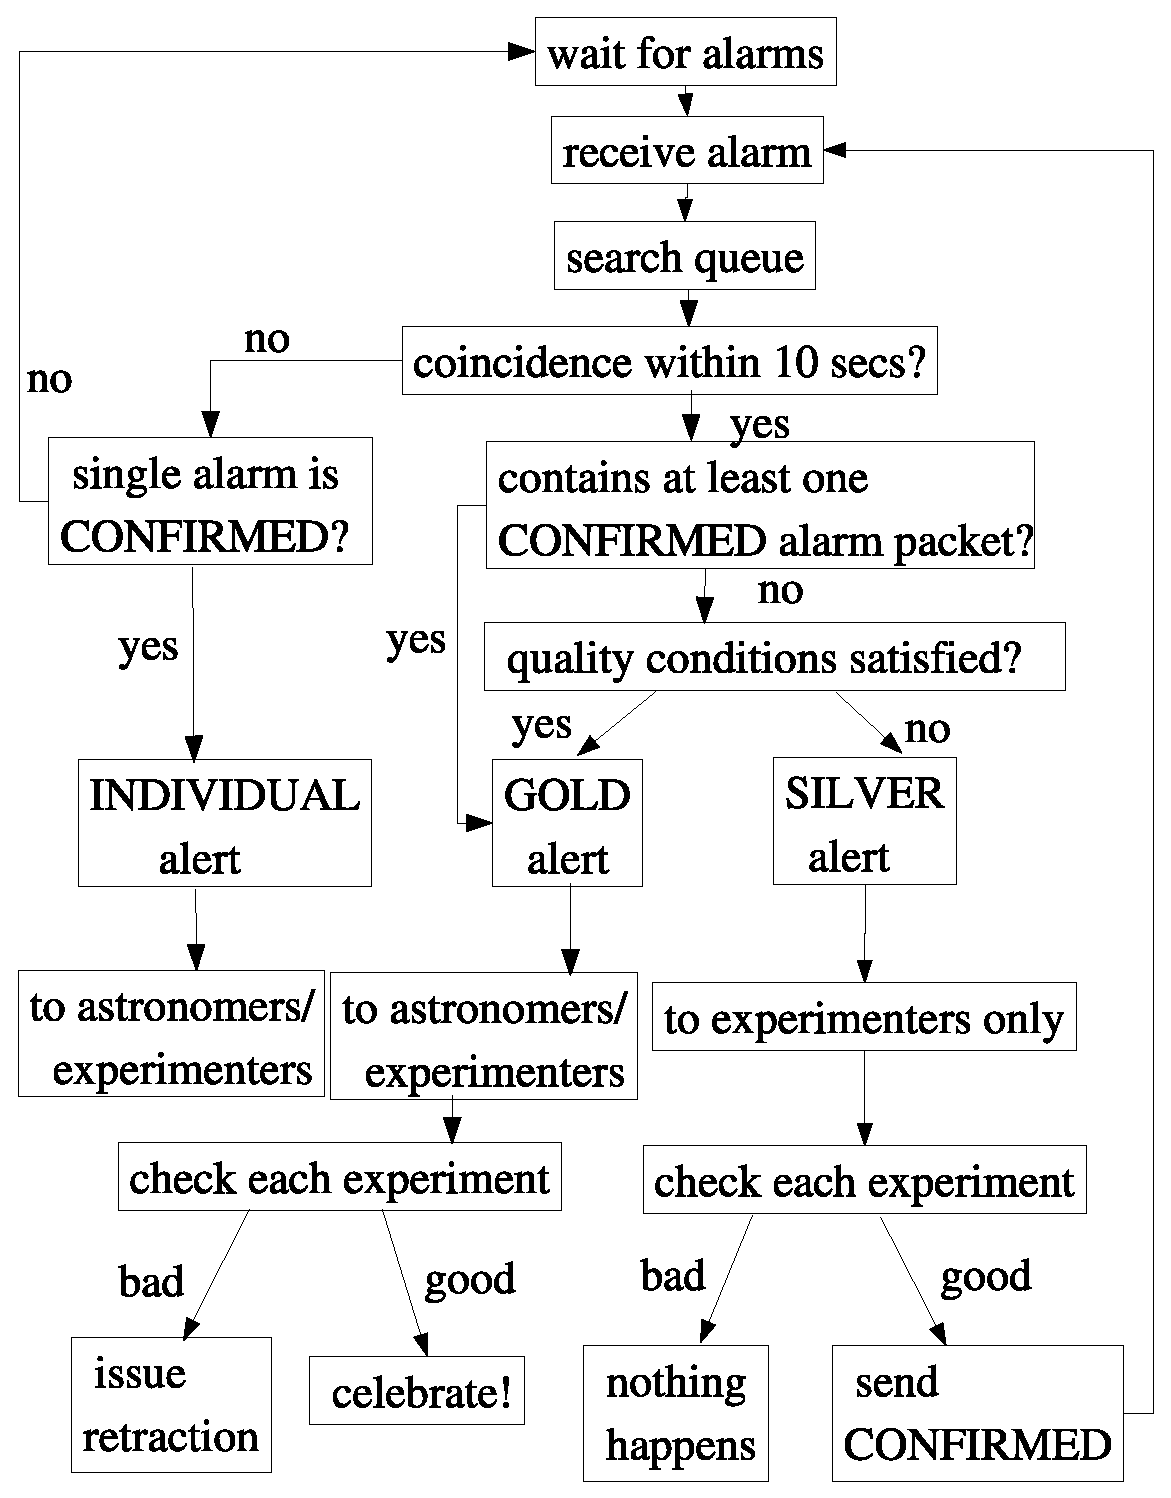
\includegraphics[width=0.68\textwidth]{snews_flowchart}
		\caption[SNEWS Flowchart]{\bf SNEWS Flowchart.\rm }
		\label{fig:flowchart}
		\vspace{0.0in}
	\end{wrapfigure}
	\filler


%-----------------------------------------------------------------------------
%-----------------------------------------------------------------------------
			
			\cleardoublepage
			%-----------------------------------------------------------------------------
%
%          PHYSICS  M.S.     THESIS
%          JUSTIN A. VASEL
%
%          This began as the template offered by the University of Minnesota, 
%          but I've made a few changes here and there...  
%
%          -->  halo.tex
%
%-----------------------------------------------------------------------------


\chapter{Helium and Lead Observatory}
	\label{halo_chapter}

	\begin{quoting}
		\noindent \large ``Astronomically Patient" \normalsize

		--- The HALO Collaboration
	\end{quoting}

	\chapterIntro{B}{uried 6,800 feet below ground,} SNOLAB is the deepest laboratory in the world. SNOLAB is located near Sudbury, Ontario, Canada in the Vale Creighton Mine. Originally, the laboratory consisted of just one experiment, the Sudbury Neutrino Observatory (SNO). Due to the success of SNO in shedding light on the solar neutrino problem, the laboratory expanded and now is home to a handful of neutrino and dark matter experiments. The Helium and Lead Observatory (HALO) is one of the experiments that calls SNOLAB its home. 

	The HALO experiment is currently in the final stages of development. When it is complete, HALO will continuously search for the distinct neutrino signal produced during a galactic supernova as a member of SNEWS. HALO is unique in that it is the only neutrino experiment whose primary objective is to detect supernova neutrinos.

	\begin{figure}[H]
		\includegraphics[width=\textwidth]{halo_diagram}
		\caption[The HALO Detector]{\bf Schematic of the HALO detector design. \rm The lead bores are shaded green. The \he proportional counters are shaded blue.}
		\label{fig:halo}
	\end{figure}

	The HALO detector consists of \ \SI[mode=text]{76}{tons} of lead and 128 \he neutron detectors. The lead serves as the interaction medium and is sectioned in blocks. Each block of lead has a bore through the middle of it within which sit four \he neutron detectors \nolinebreak (\FIG \ref{fig:halo}).

	Because galactic supernovae only occur two or three times each century\cite{sn_rates}, HALO is designed with longevity in mind. Once completed, the experiment will be highly automated and relatively inexpensive to maintain, allowing it to remain in operation for decades. 



	%% SECTION : LEAD AS AN INTERACTION MEDIUM
	\section{Lead as a Interaction Medium}

	HALO is the only neutrino experiment that uses lead as an interaction medium. Lead was chosen because it was economical, available, and efficiently delivers neutrons to the \he neutron counters in which detection actually occurs. Lead has a relatively high neutrino interaction cross section which results in the production of neutrons\cite{Engel2003}. These interactions are described as neutral current (NC), which are moderated by the $\HepParticle{\PZzero}{}{}$ boson (\EQ \ref{eq:nc}), or charged current (CC), which are moderated by the $\HepParticle{\PWpm}{}{}$ bosons (\EQS \nolinebreak \ref{eq:nue_cc}, \nolinebreak \ref{eq:nue_bar_cc})\footnote{A fourth type of neutrino interaction is elastic scattering (ES) in which a neutrino scatters off of an electron (\HepProcess{\HepParticle{\Pnue}{}{} + \HepParticle{\Pelectron}{}{} \to \HepParticle{\Pnue}{}{} + \HepParticle{\Pelectron}{}{}}). Some neutrino detectors are sensitive to this type of interaction, but HALO is not because it cannot detect electrons.}.

		\begin{align}
			\quad \textbf{Neutral Current} \qquad &\HepProcess{\HepParticle{\Pneutrino}{}{} + \text{Pb} \to \HepParticle{\Pneutrino}{}{*} + \text{Pb}^*} \label{eq:nc} \\
			\quad \textbf{$\HepParticle{\Pnue}{}{}$ Charged Current} \qquad &\HepProcess{\HepParticle{\Pnue}{}{} + \text{Pb} \to \HepParticle{\Pelectron}{}{} + \text{Bi}^*} \label{eq:nue_cc} \\
			\quad \textbf{$\HepParticle{\APnue}{}{}$ Charged Current} \qquad &\HepProcess{\HepParticle{\Pnue}{}{} + \HepParticle{\Pproton}{}{} \to \HepParticle{\Ppositron}{}{} + \HepParticle{\Pneutron}{}{}} \label{eq:nue_bar_cc}
		\end{align}

		\begin{figure}[H]
			
\includegraphics[width=\textwidth]{total}
			\caption[Neutrino Detector Sensitivities]{\bf Neutrino detector sensitivities. \rm Since HALO is the first experiment to lead as an interaction medium, it will offer unique insight into the $\HepParticle{\Pnue}{}{}$ charged current channel.}
			\label{fig:sensitivities}
		\end{figure}

	In NC interactions, a neutrino of any flavor strikes a lead nucleus and excites it. When the nucleus de-excites, zero, one, or two neutrons are produced ($\HepProcess{\text{Pb}^* \to \text{Pb} + \HepParticle{\Pphoton}{}{} + \text{neutrons}}$). In $\HepParticle{\Pnue}{}{}$ CC interactions, an electron neutrino interacts with a neutron in the lead nucleus, producing an electron and bismuth in an excited state. Again, the nucleus de-excites and produces zero, one, or two neutrons ($\HepProcess{\text{Bi}^* \to \text{Bi} + \HepParticle{\Pphoton}{}{} + \text{neutrons}}$).

	The third possible interaction, $\HepParticle{\APnue}{}{}$ CC, is highly suppressed due to ``pauli blocking.'' The excess of neutrons in lead makes it less likely that neutron will be produced because many of the low-energy states are already filled, and neutrons are fermionic particles that are subject to the Pauli exclusion principle. 

	\begin{wrapfigure}{l}{0.3\textwidth}
		\includegraphics[width=0.3\textwidth]{lead}
		\caption[Schematic of Lead Blocks]{\bf Schematic of lead blocks. \rm}
		\label{fig:lead}
		\vspace{-0.1in}
	\end{wrapfigure}
	The lead blocks were originally used in the Deep River cosmic ray experiment. The lead is stacked in alternating rows of four and five (\FIG \ref{fig:halo}) and each row runs 3 meters deep. This geometry was chosen to maximize the number of lead blocks used while being confined to the relatively small space that HALO is given in SNOLAB. HALO makes use of 76 tons of lead; 864 blocks in total.

	The lead blocks were painted to minimize health risks associated with exposure to lead and to minimize contamination of the SNOLAB environment. The type of paint used was meticulously chosen based on several factors, including its resistance to peel or rust, its neutron-capture cross section, and its containment of radioactive isotopes that could increase background noise in the detector\cite{Shantz2010}.



	%% SECTION : 3HE PROPORTIONAL COUNTERS
	\section{\he Proportional Counters}

	The neutrons produced from nuclear de-excitation of either lead or bismuth pass into one of the 128 proportional detectors (\FIG \ref{fig:ncd}) which are filled with a gaseous mixture of \he and CF$_4$ (85/15 by pressure) at a pressure of \SI[mode=text]{2.5}{atm}. The neutrons are captured on \he shortly after entering the tube by the following reaction:
	\begin{equation}
		\HepProcess{^3\text{He} + \HepParticle{\Pneutron}{}{} \to \HepParticle{\Pproton}{}{} + {}^3\text{H} + \ekeV{764}}
	\end{equation}
	Of the \ekeV{764} released from the reaction, \ekeV{573} is the kinetic energy of the proton and \ekeV{191} is the kinetic energy of the triton. The production of these charged particles ionizes the nearby gas, producing ion pairs that are accelerated in opposite directions by a coaxial anode and cathode. The electric field near the anode is strong enough to allow secondary ionization of the surrounding gas by the accelerating electrons. This produces a cascade of ionization that is ultimately collected on the anode. The amount of charge collected at the anode is proportional to the original number of ion pairs. 

	\begin{figure}[H]
		\includegraphics[width=\textwidth]{ncd}
		\caption[Technical Diagram of \he Proportional Counter]{\bf Technical diagram of \he proportional counter. \rm The counters were originally used in Phase III of the SNO experiment, but have been refitted with new endcaps for use in HALO.}
		\label{fig:ncd}
	\end{figure}

	The spectrum of neutron energies does not have a single sharp peak at \ekeV{764}, however. Instead, the spectrum has two distinct shoulders to the left of the peak (\FIG \nolinebreak \ref{fig:neutron_spectrum}). These shoulders are artifacts of the ``wall effect.'' The wall effect occurs when neutron capture happens very close to the detector wall. When the proton and triton are created, one of them may collide with the wall of the detector or be absorbed by it entirely, reducing the total kinetic energy detected by the counter.

	\begin{figure}[H]
		\centering
		\includegraphics[width=0.9\textwidth]{neutron_spectrum}
		\caption[Example Neutron-Capture Spectrum]{\bf \he neutron-capture spectrum from $^{24}$Na calibration\rm \cite{Search2011}. The neutron peak is clearly located at \ekeV{764}, but there also exist shoulders that terminate at \ekeV{573} and \ekeV{191} due to some of the triton's or proton's energy (respectively) being lost due to collisions with the walls of the counter.}
		\label{fig:neutron_spectrum}
	\end{figure}

	Of course, the neutron spectrum is the end result of analyzing the current signals generated by the cascading electrons near the anode, which will be discussed in greater detail in \SEC \ref{sec:electronics}. The proton-triton pair move away from each other in some orientation relative to the anode at the center of the tube. The particular orientation influences the shape of the current pulse that is collected at the anode. If, when created, the proton is moving toward the anode, then the triton is moving away from the anode and the current pulse from the proton will arrive before that of the triton. If the proton and triton are produced in such a way that they both move parallel to the anode wire, then their current pulses will arrive at the anode simultaneously. 

	\begin{figure}[H]
		\centering
		\includegraphics[width=0.9\textwidth]{capture}
		\caption[\he Neutron Capture Schematic]{\bf \he Neutron capture schematic\rm \cite{Search2011}. The proton-triton pair are produced and move in opposite directions. The proton and triton peaks may be separated in time by an amount determined by their orientation in the counter.}
		\label{fig:capture}
	\end{figure}

	%% SECTION : NEUTRON BACKGROUNDS AND NOISE
	\section{Neutron Backgrounds and Noise}
	SNOLAB is better than any other laboratory when it comes to sheilding. The \SI[mode=text]{6800}{feet} of rock that sit above it is the equivalent of \SI{6000}{\meter} of water. That notwithstanding, there is still background flux of both fast and thermal neutrons produced by radioactive decays and cosmic ray muon interactions within the surround rock. The flux of thermal and fast neutrons in SNOLAB has been measured to be \SI[mode=text]{4100}{neutrons.m^{-2}.day^{-1}} and \SI[mode=text]{4000}{neutrons.m^{-2}.day^{-1}} respectively\cite{handbook}. 

	To ensure that HALO will maintain the false-alarm rate required for participation in SNEWS (see \SEC \ref{sec:snews_positive}), shielding must be placed around the detector to block as much of the neutron background as possible. 

	\plan{MISSING CHUNK HERE ABOUT SHEILDING} 
 
	The proportional counters are very effective as long as ionization is induced by neutron capture events only. Collisions within\he gas can excite molecules without ionizing them, leading to the emission of a photon when the molecule de-excites. The photons can then go on to cause ionization elsewhere in the detector. This is the reason for the \he/CF$_4$ mixture. The CF$_4$ provides stopping power for ionizing particles, substantially reducing the effect.

	The outer shell of the\he counter is composed of ultra-pure nickel. The walls are only \SI{380}{\micron} thick and were produced in a uniform way through the process of chemical vapor deposition. Despite the purity of the detector material, there are trace amounts of radioactive nuclei that contribute to noise in the signal. The most common byproduct of radioactive decays are $\alpha$ particles. The $\alpha$ particles can interact with other elements resulting in the production of a neutron. Fortunately, $\alpha$ particles have charge and are very heavy and so they have a very short range. This prevents them in many cases from arriving at the detector wall with sufficient energy to initiate radioactive decay. 

	The few neutrons that are produced by interactions with $\alpha$ particles have energies that are a couple tens of \eMeV{}, making them indistinguishable from neutrons produced by supernova neutrino interactions. A study of these $\alpha$ backgrounds found that the rate of neutron-producing $\alpha$ particles was $21.9^{+1.1}_{-1.0}$ per day and is considered negligable\cite{Shantz2010}. 

	Gamma rays are another source of noise and are produced through nuclear decays of uranium and thorium found in the paint that coats the lead blocks. Uranium and thorium decay via $\alpha$ or $\beta$ emission, but the decay of daughter nuclei can produce gammas. These photons can interact with electrons via Compton scattering and cause the electrons to move. Multiple scattering effects may imbue the electrons with enough energy to survive being cut by detector electronics, resulting in the false count of a neutron. Simulations\cite{Shantz2010} and HALO data show that the energy of these gamma-induced counts tends to be less than a few \eMeV{}, making them easily distinguishable from the neutrino-induced neutron signal.

 	%% SECTION : DETECTOR ELECTRONICS AND DATA FLOW
	\section{Detector Electronics and Data Acquisition}
	\label{sec:electronics}
		\filler


%-----------------------------------------------------------------------------
%-----------------------------------------------------------------------------
			
			\cleardoublepage
			%-----------------------------------------------------------------------------
%
%          PHYSICS  M.S.     THESIS
%          JUSTIN A. VASEL
%
%          This began as the template offered by the University of Minnesota, 
%          but I've made a few changes here and there...  
%
%          -->  halo2.tex
%
%-----------------------------------------------------------------------------


\chapter{The Road to Full Operation}
	\label{halo2_chapter}

	\begin{quoting}
		\noindent \large ``For tomorrow belongs to the people who prepare for it today." \normalsize

		--- African Proverb
	\end{quoting}

	\chapterIntro{I}{arrived at SNOLAB to begin work on HALO in July of 2012.} Construction of the detector hardware had finished not long before that and the detector had been running and collecting data since May of 2012. However, HALO was far from being ready to do its job. Many vital components were missing: SNEWS alert triggers were not developed, hardware redundancy was not in place, there was no way to remotely monitor the hardware, and the detector had not yet been calibrated. 

	My job at HALO was not singularly data analysis nor theoretical research nor computer simulation. My contribution to the experiment was more vague and arguably more involved: to help the collaboration move through this laundry list of tasks in a timely manner so that HALO will be ready to serve its purpose before the next galactic supernova occurs. In this chapter, I will discuss my involvement in preparing the Helium and Lead Observatory for full operation.

	\section{Identifying Faulty{}\he Counters}
		As mentioned in \CHP \ref{halo_chapter}, the{}\he proportional counters were donated to HALO by the decommissioned SNO experiment. Only 128 counters are required for HALO, which left us with a couple dozen extra to be kept on reserve in case a counter in the detector for whatever reason needs to be replaced. The neutron spectrum for each counter currently in the detector had been carefully examined to ensure the active counters were behaving as expected, but the extra counters had not yet been so thoroughly vetted. It was known that some of the counters were filled with $^4$He gas, which cannot be used in the detection of neutrons. The SNO experiment used these as a control group and they got mixed in with the{}\he counters when they were delivered to HALO. 

		To identify the $^4$He counters in the group and to ensure that the{}\he counters were behaving normally, we tested each of them by collecting and examining their neutron spectrum. To avoid disrupting any of the 128 active counters in the detector during testing, we ran wiring from the storage rack to the rest of the hardware. This allowed us to test four counters at a time while the rest of the detector ran normally.

		Most counters were allowed to accumulate data for several days before inspection. A healthy{}\he counter displayed a statistically significant neutron peak located near an ADC value of 1,000\footnote{At this point, the arbitrary ADC value scale for energy had not been mapped to keV. Such a mapping depends on the peculiarities of the{}\he counter, the gains within it, and thresholds applied to it. An algorithm to perform this conversion for each counter is currently in development.} and a tall and sharp gamma peak at very low energies (\FIG \ref{fig:halo_neutron_spectra}, left). An unhealthy{}\he counter may have a broadened neutron peak or other strange artifacts in the spectrum (\FIG \ref{fig:halo_neutron_spectra}, center). A $^4$He counter would simply not have the neutron peak (\FIG \ref{fig:halo_neutron_spectra}, right).
		\begin{figure}[H]
			\includegraphics[width=\textwidth]{halo_neutron_spectra}
			\caption[Neutron Counter Response]{\bf Neutron counter response. \rm A healthy{}\he counter \emph{(left)} exhibits a sharp neutron peak and a gamma peak. An unhealthy{}\he counter \emph{(center)} also has a gamma peak, but may show a broadened neutron peak or other obscure features. A $^4$He counter \emph{(right)} features a gamma peak, but no neutron peak.}
		\label{fig:halo_neutron_spectra}
		\end{figure}

		After characterization, we identified both healthy and unhealthy{}\he counters and the $^4$He counters. \confirm{A \he counter with a gas leak will experience a decrease in gain} and manifest itself as a distorted neutron spectrum. We suspected that any unhealthy spectra we found would be due to such a leak, but after finding several of these, we began to wonder if there was another explanation. It was a symptom worthy of further investigation, in case it could affect healthy{}\he detectors down the road.
	\section{DAQ Software Development}
		\filler
	\section{Remote Monitoring}
		\filler
	\section{Current Status and Future Work}
		\filler


%-----------------------------------------------------------------------------
%-----------------------------------------------------------------------------

		% // Conclusion
			\cleardoublepage
			%-----------------------------------------------------------------------------
%
%          PHYSICS  M.S.     THESIS
%          JUSTIN A. VASEL
%
%          This began as the template offered by the University of Minnesota, 
%          but I've made a few changes here and there...  
%
%          -->  conclusion.tex
%
%-----------------------------------------------------------------------------


\chapter{Conclusion and Discussion}
	\label{conclusion_chapter}
	\vspace{-0.2in}

	\begin{quoting}
		\noindent \large ``It is a capital mistake to theorize before one has data. Insensibly one begins to twist facts to suit theories, instead of theories to suit facts." \normalsize

		--- Sir Arthur Conan Doyle
	\end{quoting}

	\filler


%-----------------------------------------------------------------------------
%-----------------------------------------------------------------------------



	%%%%%%%%%%%%%%%%%%%%%%%%%%%%%%%
	%   //  BIBLIOGRAPHY          %
	%%%%%%%%%%%%%%%%%%%%%%%%%%%%%%%

		% // Style provided by the University of Minnesota
		\bibliographystyle{hunsrt}

		% // Read BibTeX file
		\bibliography{thesis}



	%%%%%%%%%%%%%%%%%%%%%%%%%%%%%%%
	%   //  APPENDICES            %
	%%%%%%%%%%%%%%%%%%%%%%%%%%%%%%%

		\appendix
		%-----------------------------------------------------------------------------
%
%          PHYSICS  M.S.     THESIS
%          JUSTIN A. VASEL
%
%          This began as the template offered by the University of Minnesota, 
%          but I've made a few changes here and there...  
%
%          -->  app_glossary.tex
%
%-----------------------------------------------------------------------------


\chapter{Glossary and Acronyms}
\label{app_glossary}

\scaps{Care has been taken in this thesis} to minimize the use of jargon and
acronyms. It is my personal philosophy that ideas should be expressed in the 
simplest way possible, avoiding the convoluted use of jargon whenever possible. 
Unfortunately, this cannot always be achieved.  This appendix defines jargon 
terms in a glossary, and contains a table of acronyms and their meaning.


%-------------------------------------------------------------------------------
%    //  G L O S S A R Y
%===============================================================================
\section{Glossary}
\label{jargonapp}
%-------------------------------------------------------------------------------
\begin{itemize}

\item \textbf{Lepton} -- A class of fermionic particles, including the electron, muon, tau and their associated neutrinos and antiparticles.

\end{itemize}


%-------------------------------------------------------------------------------
%    //  A C R O N Y M S
%===============================================================================
\section{Acronyms}
\label{acronymsec}
%-------------------------------------------------------------------------------

%\setlength\LTleft{0pt}
%\setlength\LTright{0pt}

\begin{longtable}{|p{0.25\textwidth}|p{0.75\textwidth}|}
\caption{Acronyms} \label{Acronyms} \\

\hline
Acronym & Meaning \\
\hline \hline
\endfirsthead

\multicolumn{2}{l}%
{{\bfseries \tablename\ \thetable{} -- continued from previous page}} \\
\hline
Acronym & Meaning \\
\hline \hline
\endhead

\hline \hline \multicolumn{2}{|r|}{{Continued on next page}} \\ \hline
\endfoot

\hline \hline
\endlastfoot

HALO & Helium And Lead Observatory \\
SNEWS & SuperNova Early Warning System \\
PMNS & Pontecorvo–Maki–Nakagawa–Sakata 

\end{longtable}


%-------------------------------------------------------------------------------
%-------------------------------------------------------------------------------






%-------------------------------------------------------------------------------
%    //  E N D   D O C U M E N T
%===============================================================================
	\end{document}





